\documentclass{article}
\usepackage{graphicx} % new way of doing eps files
\usepackage{listings} % nice code layout
\usepackage[usenames]{color} % color
\definecolor{listinggray}{gray}{0.9}
\definecolor{graphgray}{gray}{0.7}
\definecolor{ans}{rgb}{1,0,0}
\definecolor{blue}{rgb}{0,0,1}
% \Verilog{title}{label}{file}
\newcommand{\Verilog}[3]{
  \lstset{language=Verilog}
  \lstset{backgroundcolor=\color{listinggray},rulecolor=\color{blue}}
  \lstset{linewidth=\textwidth}
  \lstset{commentstyle=\textit, stringstyle=\upshape,showspaces=false}
  \lstset{frame=tb}
  \lstinputlisting[caption={#1},label={#2}]{#3}
}


\author{Cameron Anderson}
\title{Class Report 2: Block Memory}

\begin{document}
\maketitle

\section{Introduction}
The goal of this project was to use the seven-segment display and binary switches to read and write to and from the block memory within the Nexys 4 DDR prototyping board. For this project, the data and address registers are each 32 bits. The seven-segment display has 8 digits and can display the full range of hexidecimal digits at each of the 8 locations. With only 16 switches, the registers will need to be divided into MSB and LSB registers to read in the switches.

\section{Experimental Plan}
Figure~\ref{fig:blockmemstatemachine} on page~\pageref{fig:blockmemstatemachine} shows the top level state machine that was used to transition between collecting the address and reading and writing to and from Block RAM. Because the registers were each 32 bits and there were only 16 switches, collecting the values through the switches had to be broken up into MSB and LSB states. This did not, however, affect the read from the BRAM because the seven segment display was able to read 8 hexidecimal digits equalling a total of 32 binary bits. The state machine transitions were completed by four buttons on the Nexys 4 DDR board. The buttons were arranged nicely in the order of the state machine. The top button was used to set first the MSB of the address and then the LSB of the address. On the next row down, the outside buttons were used to transition to the next state. The left button on the middle row was used to select the read function to display the BRAM's contents at the previously selected address. The right button on the middle row was used to select the write function. This button was used twice in succession after changing the switches to match the MSB 2 bytes of what was to be written to the previously selected address first and then similarly the LSB 2 bytes of the data. In addition to the state machine, Chu provided a module for displaying hexidecimal digits to the seven segment display but only the rightmost 4 digits. This was altered for this project to include all 8 digits of the seven segment display to read all 32 bits from an address in BRAM.
\begin{figure}
\begin{center}
\caption{State Machine for using Block Memory}\label{fig:blockmemstatemachine}
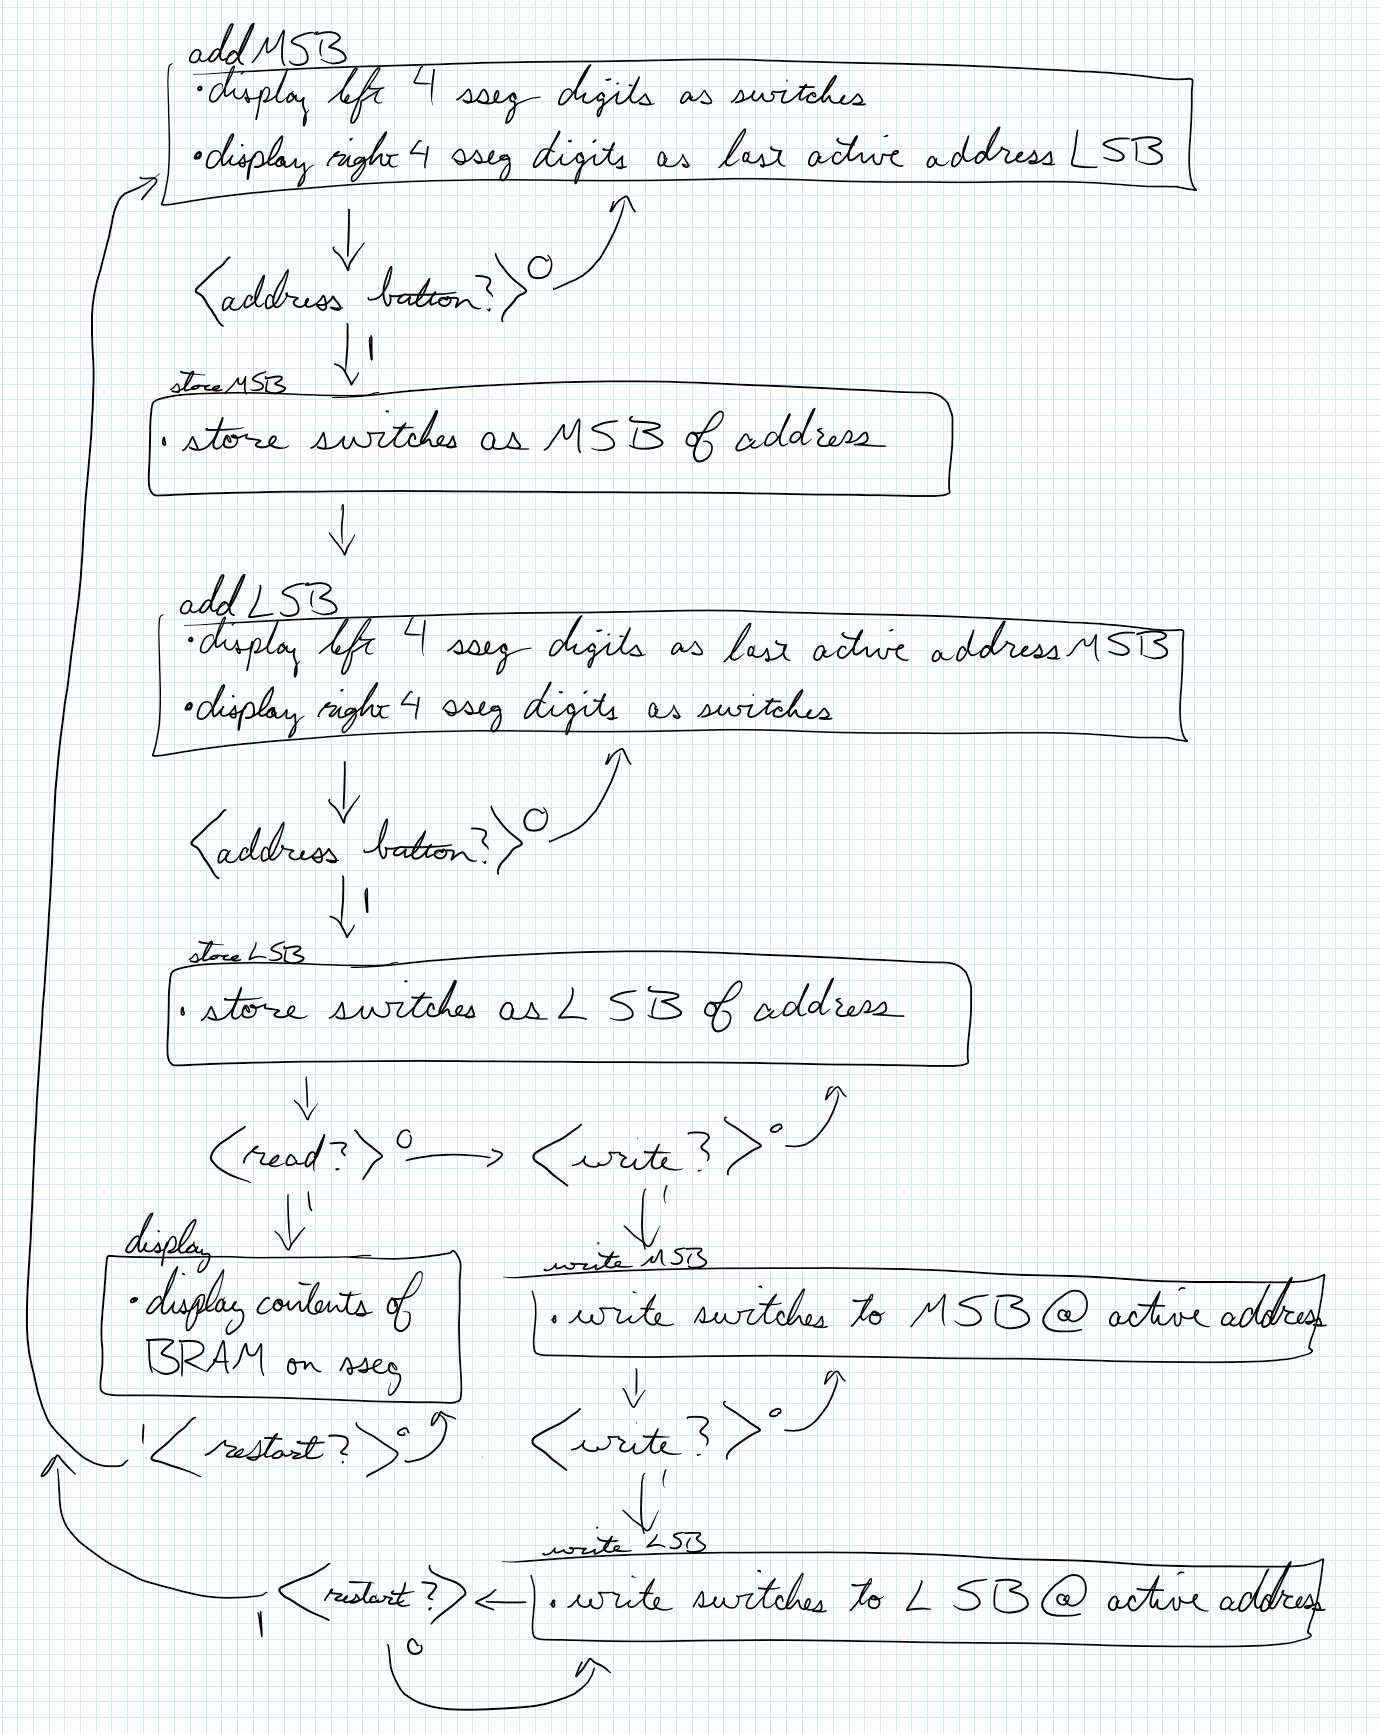
\includegraphics[width=0.9\textwidth]{blockmemstatemachine.jpg}
\end{center}
\end{figure}

\section{Conclusion}
This main components of this project were the read/write state machine and the BRAM instantiation. The read/write state machine used four buttons: one for loading in two bytes of the address at a time, another for reading from that address, another for writing to that address two bytes at a time, and a fourth for restarting the process. The read functionality only required one state because the eight digit seven-segment display is able to display eight hexidecimal digits for a total of 32 bits. The address and writes each required an MSB and then LSB states in the state machine to load all 32 bits since only 16 switches are available at a time on the Nexys 4 DDR.

\section{Appendix}

\Verilog{System Verilog code for the BRAM state machine top module}{code:rwstatemachine}{rd_wr_state_machine.sv} 

\Verilog{Verilog code for the BRAM wrapper}{code:BRAMwrapper}{BRAM_wrapper.v} 

\Verilog{System Verilog code for the hexidecimal display mux}{code:hexmux}{ch04_17_disp_hex_mux.sv} 

\end{document} 